\section{Introduction to controlling a detector}
A robust, well-defined control system is a compulsory element for every complex experimental setup, especially in radiation-controlled areas. To ensure the safe operation of a detector subsystem, automation processes are commonly implemented (e.g., in the form of a Finite State Machine\footnote{A state of the Finite State Machine is clearly defined at any given point in time. It can move to another state by processing an input.} (\gls{FSM}) or hardware interlocks). In the \gls{STS} case, to ease the use and implementation of a control system, a fairly novel approach was used. It is primarily based on the containerization\footnote{Containerization is the packaging of software code with just the operating system libraries and dependencies required to run the code.} of different applications used to monitor and control setups. 

%\begin{figure}[!h]
%\centering
%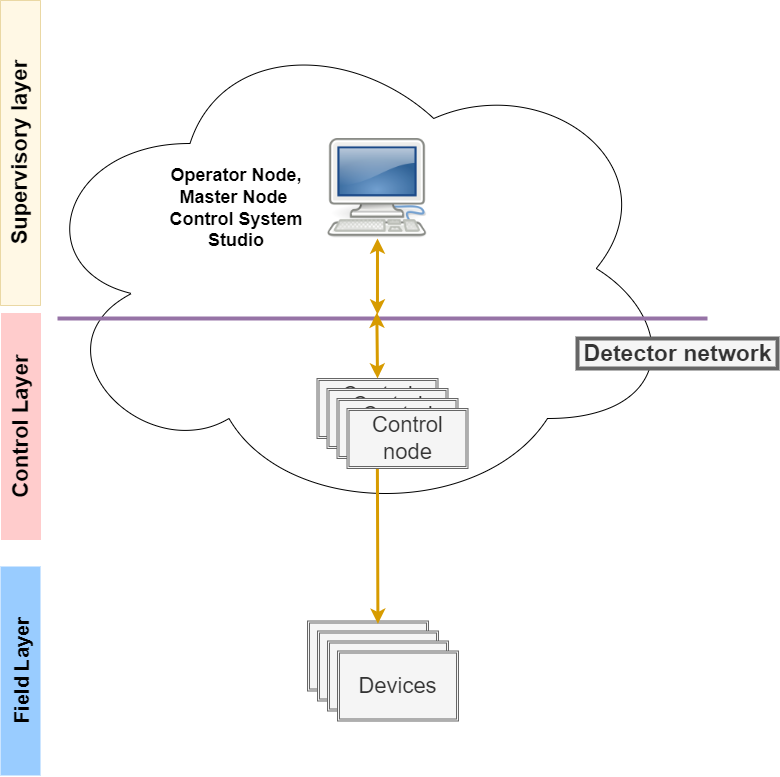
\includegraphics[width=0.55\columnwidth]{Chapter3/Controls/images/example.png}
%\caption{General detector control system architecture}
%\label{fig_DCS_arch}
%\end{figure}



A control system must provide multiple functionalities to operate effectively. These include communication between hardware and software layers, visualization of data, logging of system events, archiving of historical data, and controlling means. Control can be automated using a \gls{FSM} or performed manually, depending on the requirements of the system being controlled. The control system can be usually divided into three layers: field layer, control layer, and supervisory layer. The bottom (field) layer contains all the process sensors, actuators, and other devices that are connected to the control system via I/O boards and/or field buses. Communication between the field layer and control layer can be of almost any type compatible with the used components, i.e., Ethernet, Modbus \gls{TCP}, Profibus. The control logic is introduced in the Programmable Logic Controller (\glspl{PLC}) and so-called control nodes (single board computers etc.) in the control layer. The supervision layer or supervisory level provides the operators with means of controlling and monitoring the subsystem, for example via command line or a Graphical User Interface (\gls{GUI}) or Operator Interface (\gls{OPI})~\cite{layers}.  Typically, DCS building blocks reside in a dedicated network to avoid unnecessary cross-talk and ensure more efficient debugging.

Figure \ref{fig_arch} shows a general idea behind the \gls{STS} \gls{DCS} from the software point of view.  The master node or the central \gls{DCS} node receives data from the configuration database, which allows the preparation of subsystems for a given action (for example, for a transition into a different state). The master node will be only accessible by the \gls{DCS} experts, excluding subsystem-related personnel from performing actions on other subsystems \gls{DCS}. There are also one or more archiving nodes and control nodes, which will contain detector-specific applications. All the mentioned components allow effective control over a detector and deliver crucial operational information (alarms, events, Process Variables (\glspl{PV}) values, etc.). 

\begin{figure}[!h]
\centering
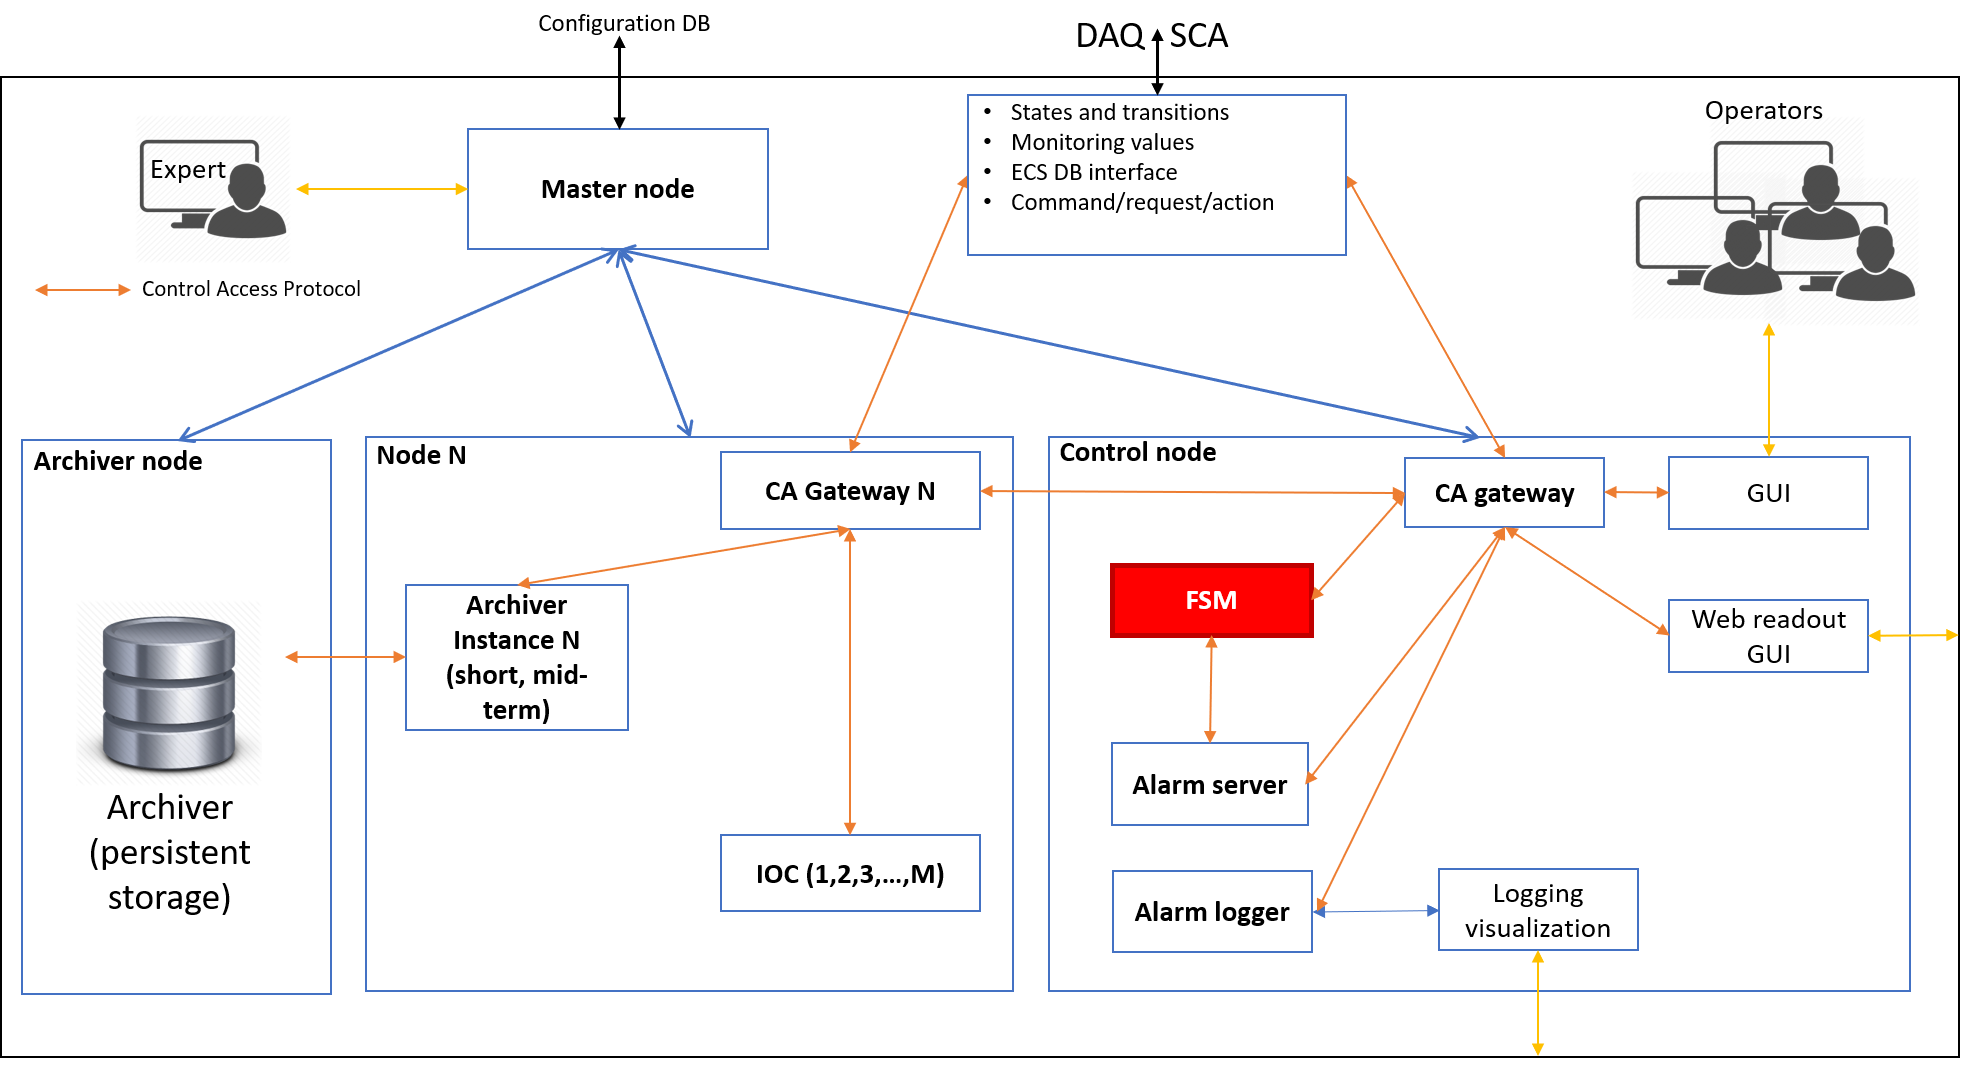
\includegraphics[width=1\columnwidth]{Chapter3/Controls/images/DCS.png}
\caption{Proposed \gls{DCS} infrastructure for the \gls{STS}. The scheme describes the most important software components including the archiver, alarm server, alarm logger, GUIs, \glspl{FSM}, and corresponding interfaces.}
\label{fig_arch}
\end{figure}
\newpage





